\documentclass[11pt,a4paper]{article}

% ── Packages ──────────────────────────────────────────────────────────────────
\usepackage[margin=1in]{geometry}
\usepackage[T1]{fontenc}
\usepackage{lmodern}
\usepackage{amsmath,amssymb}
\usepackage{graphicx}
\usepackage{array}
\usepackage[table]{xcolor}
\usepackage{booktabs}
\usepackage{tabularx}
\usepackage{caption}
\usepackage{titlesec}
\usepackage{parskip}
\usepackage{hyperref}
\usepackage{enumitem}
\usepackage{fancyhdr}
\usepackage{seqsplit}
\usepackage{tikz}
\usetikzlibrary{shapes.geometric,arrows.meta,positioning,fit,backgrounds,calc}

% ── Colours ───────────────────────────────────────────────────────────────────
\definecolor{titleblue}{RGB}{46,116,181}
\definecolor{darkblue}{RGB}{31,78,121}
\definecolor{rowgray}{RGB}{235,243,251}
\definecolor{headerblue}{RGB}{46,116,181}
\colorlet{ewublue}{darkblue}
\definecolor{nodeblue}{RGB}{224,231,255}
\definecolor{nodeindigo}{RGB}{199,210,254}
\definecolor{nodegreen}{RGB}{209,250,229}
\definecolor{nodegray}{RGB}{226,232,240}
\definecolor{codebg}{RGB}{238,242,255}

% ── Column types ──────────────────────────────────────────────────────────────
\newcolumntype{L}[1]{>{\raggedright\arraybackslash}p{#1}}
\newcolumntype{C}[1]{>{\centering\arraybackslash}p{#1}}

% ── Section formatting ────────────────────────────────────────────────────────
\titleformat{\section}{\large\bfseries\color{titleblue}}{\thesection\quad}{0em}{}
  [\color{titleblue}\titlerule]
\titleformat{\subsection}{\normalsize\bfseries\color{darkblue}}{\thesubsection\quad}{0em}{}
\titleformat{\subsubsection}{\small\bfseries\color{darkblue}}{\thesubsubsection\quad}{0em}{}
\titlespacing*{\section}{0pt}{18pt}{8pt}
\titlespacing*{\subsection}{0pt}{12pt}{4pt}

% ── Header / Footer ───────────────────────────────────────────────────────────
\pagestyle{fancy}
\fancyhf{}
\rhead{\small\color{gray}Software Requirements Specification}
\lhead{\small\color{gray}scholar-agent}
\cfoot{\small\color{gray}\thepage}
\renewcommand{\headrulewidth}{0.4pt}

\hypersetup{colorlinks=true,linkcolor=titleblue,urlcolor=titleblue,citecolor=titleblue}

% ── Code / listing box ────────────────────────────────────────────────────────
\newcommand{\code}[1]{\leavevmode{\color{darkblue}\texttt{#1}}}
% break-friendly code for long identifiers inside narrow table cells
\newcommand{\bcode}[1]{\leavevmode{\color{darkblue}\texttt{\seqsplit{#1}}}}

% TikZ base styles
\tikzset{
  box/.style={rectangle,rounded corners=3pt,draw=darkblue!60,fill=nodeblue,
              text=black,align=center,inner sep=5pt,font=\footnotesize,minimum height=8mm},
  ibox/.style={box,fill=nodeindigo},
  gbox/.style={box,fill=nodegreen},
  store/.style={cylinder,shape border rotate=90,aspect=0.25,draw=darkblue!60,
                fill=nodegray,align=center,inner sep=4pt,font=\scriptsize,minimum height=11mm},
  actor/.style={circle,draw=darkblue!70,fill=white,align=center,font=\scriptsize,inner sep=3pt},
  fl/.style={-{Stealth[length=2.2mm]},draw=darkblue!70,font=\scriptsize},
  grp/.style={rectangle,rounded corners=4pt,draw=titleblue!40,fill=titleblue!5,inner sep=8pt},
}

% ── QFD relationship legend ──────────────────────────────────────────────────
\newcommand{\qstrong}{\textcolor{titleblue}{$\bullet$}}
\newcommand{\qmed}{\textcolor{titleblue}{$\circ$}}
\newcommand{\qweak}{\textcolor{titleblue}{$\triangle$}}
\newcommand{\qpos}{\textcolor{nodegreen!70!black}{$+$}}
\newcommand{\qneg}{\textcolor{red!60!black}{$-$}}

\begin{document}

% ══════════════════════════════════════════════════════════════════════════════
% COVER PAGE
% ══════════════════════════════════════════════════════════════════════════════
\thispagestyle{empty}
\begin{center}
  \includegraphics[width=3.2cm]{logo.jpg}\\[10pt]
  {\Large\bfseries\color{ewublue} EAST WEST UNIVERSITY}\\[3pt]
  {\normalsize\bfseries\color{ewublue} Department of Computer Science and Engineering}\\[5pt]
  {\large\bfseries\color{ewublue} SOFTWARE REQUIREMENTS SPECIFICATION}\\[16pt]

  \fbox{%
    \parbox{0.85\textwidth}{%
      \centering\vspace{6pt}
      {\small\color{ewublue} Project Title}\\[6pt]
      {\large\bfseries scholar-agent: An Autonomous Scholarship and PhD\\
        Application Platform}\\[8pt]
      {\small\color{ewublue} Course: CSE 412 (Software Engineering)}\\[4pt]
    }%
  }
\end{center}

\vspace{16pt}
{\bfseries\color{ewublue} Submitted By}\\[6pt]
\renewcommand{\arraystretch}{1.4}
\begin{tabular}{|p{0.5\linewidth}|p{0.38\linewidth}|}
\hline
\rowcolor{ewublue!80}\textcolor{white}{\textbf{Student Name}} & \textcolor{white}{\textbf{Student ID}} \\
\hline
Md. Tamim Hasan Saykat       & 2022-1-60-289 \\ \hline
Md. Mahamudur Rahman Maharaz & 2022-3-60-182 \\ \hline
Naima Islam                  & 2022-3-60-215 \\ \hline
\end{tabular}

\vspace{14pt}

\vspace{16pt}
{\bfseries\color{ewublue} Submitted To}\\[6pt]
\noindent{\bfseries Yasin Sazid}\\
Lecturer\\
Department of Computer Science and Engineering, East West University

\vspace{10pt}
{\bfseries\color{ewublue} Requirements Engineering Methodology}\\[4pt]
\noindent IEEE 830 conventions for requirements specification; stakeholder analysis and
requirements elicitation per Pressman, \textit{Software Engineering: A Practitioner's
Approach}, Chapter 5 (Understanding Requirements); Quality Function Deployment / House of
Quality per Cohen, \textit{Quality Function Deployment: How to Make QFD Work for You} (1995).

\vspace{6pt}
{\small\itshape Note: this document supersedes the team's earlier Software Design Document
submission and restructures the same project around the SRS deliverable format.}

\vfill
\begin{center}\small Department of Computer Science and Engineering\end{center}
\newpage

% ══════════════════════════════════════════════════════════════════════════════
\section{Introduction}

\subsection{Project Overview}
\textbf{User story.} \emph{As a final-year student hunting for a fully funded PhD or
scholarship, I want one account where I can discover opportunities that actually match my
profile, understand why each one fits, track every application to its deadline, and get a
factually grounded cold email and Statement of Purpose drafted for me --- so that I stop
losing offers to spreadsheet chaos, dozens of open browser tabs, and hours of repetitive,
error-prone writing.}

scholar-agent is a web platform for finding, tracking, and completing funded study
opportunities (scholarships and PhD positions) from a single account. It has two cooperating
parts. A \textbf{discovery engine} searches the live web, extracts structured opportunity
records, ranks them against the user's CV, and drafts application materials. A \textbf{system
of record}, which is the web application itself, stores accounts, tracks each application
through a status pipeline, manages professor outreach, and hosts a writing practice module.

The split between these two parts is deliberate. The discovery engine answers the question
\emph{``what opportunities exist?''} and writes to a shared knowledge base built from a graph
store and a vector store. The system of record answers \emph{``what is this user doing about
them?''} and writes to a per-user relational database. This separation is the central
requirement-driving decision of the system, and later sections of this SRS refer back to it.

\subsection{Purpose and Scope}
\textbf{Purpose.} This Software Requirements Specification (SRS) defines the functional,
non-functional, and quality-driven requirements that scholar-agent must satisfy. It is the
contract between the stakeholders identified in \S\ref{sec:stakeholders} and Group H's
development team: it states \emph{what} the system must do, not \emph{how} it is built
internally, and it is the basis against which the finished platform is evaluated for the
CSE 412 course deliverable.

\textbf{In scope.} Account creation and authentication; CV ingestion and profile extraction;
web-scale discovery and extraction of scholarship/PhD opportunities; profile-to-opportunity
matching with an explainable score; a personal application-tracking pipeline with a
requirement checklist; grounded drafting of cold emails and Statements of Purpose; a
professor-outreach log; a unified calendar export; a standing watchlist that is re-searched
automatically; and a writing-practice module with criterion-level feedback.

\textbf{Out of scope.} scholar-agent does not submit applications through third-party
university or funder portals on the user's behalf; it does not guarantee admission or
funding outcomes; it does not process payments, visas, or legal immigration paperwork; and
it is not a general-purpose job board.

\subsection{Stakeholders}\label{sec:stakeholders}
Six stakeholder groups shape this specification, spanning the student who uses the product,
the team that builds and is graded on it, the people the product writes to on the student's
behalf, and the infrastructure the product depends on. Each is analysed in
\S\ref{sec:stakeholder-analysis}, and every requirement in \S\ref{sec:reqlist} traces back to
at least one of them.

% ══════════════════════════════════════════════════════════════════════════════
\section{Requirements Engineering Process}

\subsection{Stakeholder Needs \& Analysis}\label{sec:stakeholder-analysis}

\subsubsection{Primary and Secondary Stakeholders}
\renewcommand{\arraystretch}{1.3}
\begin{tabularx}{\linewidth}{|L{3.2cm}|C{1.9cm}|X|}
\hline
\rowcolor{headerblue}\textcolor{white}{\textbf{Stakeholder}} & \textcolor{white}{\textbf{Type}} & \textcolor{white}{\textbf{Interest / Need}} \\
\hline
Student Applicant (end user) & Primary & Wants qualified opportunities surfaced automatically, deadlines never missed, and application materials drafted without misrepresenting them. \\
\rowcolor{rowgray}
Development Team (Group H) & Primary & Builds, tests, and is graded on the platform; needs requirements precise enough to design and estimate against. \\
Course Instructor / Evaluator (Yasin Sazid) & Secondary & Assesses whether the specification is complete, traceable, and technically sound per the CSE 412 rubric. \\
\rowcolor{rowgray}
Target Professors \& University Admissions Offices & Secondary & Receive the drafted outreach; need it accurate, non-generic, and free of fabricated claims about them. \\
LLM / API Providers (Groq, Gemini, Ollama pool) & Secondary & Supply inference capacity within free-tier limits; the system must respect their rate limits and terms. \\
\rowcolor{rowgray}
Future Maintainers / Open-Source Contributors & Secondary & Need the system extensible (new providers, agents, resources) without touching existing, working code. \\
\hline
\end{tabularx}

\subsubsection{Methods Used for Requirement Elicitation}
Because scholar-agent is a course project built by students who are themselves in the
target audience, elicitation combined lightweight, low-cost techniques rather than a formal
enterprise process:
\begin{itemize}[leftmargin=14pt,itemsep=3pt]
  \item \textbf{Self-elicitation as proxy end-users.} All three team members are actively
    applying, or have applied, for funded scholarships and PhD positions, so first-hand
    frustration with manual search, tracking, and drafting was captured directly as
    requirements rather than inferred second-hand.
  \item \textbf{Informal interviews.} Short, unstructured conversations with peer applicants
    and labmates in the team's research group surfaced recurring pain points --- deadline
    tracking across spreadsheets, uncertainty about eligibility, and the time cost of writing
    a unique cold email per professor.
  \item \textbf{Competitor and workflow analysis.} Existing scholarship databases (DAAD,
    Fulbright, Erasmus) and generic chatbot-assisted drafting were walked through end to end
    to identify what they leave the applicant to do manually; those gaps became functional
    requirements.
  \item \textbf{Iterative prototyping with supervisor feedback.} Early wireframes and a
    working pipeline prototype were reviewed with the course instructor, and the requirement
    list was revised in response.
  \item \textbf{Domain document review.} Pressman's requirements-engineering checklist
    (Ch.\,5) was used to sanity-check the draft requirement list for completeness,
    consistency, and verifiability before it was finalised below.
\end{itemize}

\subsection{List of Requirements}\label{sec:reqlist}

\subsubsection{Functional Requirements}
\renewcommand{\arraystretch}{1.25}
\begin{tabularx}{\linewidth}{|C{1.35cm}|X|}
\hline
\rowcolor{headerblue}\textcolor{white}{\textbf{ID}} & \textcolor{white}{\textbf{Requirement}} \\
\hline
\mbox{FR-1} & A visitor can register and authenticate; all data is private to the account. \\
\rowcolor{rowgray}
\mbox{FR-2} & A user uploads or pastes a CV; the system extracts a structured profile. \\
\mbox{FR-3} & The system searches the web from free-text topics and extracts structured opportunity records. \\
\rowcolor{rowgray}
\mbox{FR-4} & Extracted opportunities are persisted to the knowledge base and de-duplicated by content identity. \\
\mbox{FR-5} & A user browses and filters the catalog and saves opportunities into a personal pipeline. \\
\rowcolor{rowgray}
\mbox{FR-6} & The system ranks opportunities against a profile and returns a score with a rationale. \\
\mbox{FR-7} & A user tracks each application through a status pipeline with a requirement checklist. \\
\rowcolor{rowgray}
\mbox{FR-8} & The system drafts a grounded cold email and Statement of Purpose per application, and persists them. \\
\mbox{FR-9} & A user maintains a professor-outreach record with a message thread and follow-up dates. \\
\rowcolor{rowgray}
\mbox{FR-10} & The system exports all deadlines and follow-ups as an importable calendar (.ics). \\
\mbox{FR-11} & A user keeps a watchlist of standing interests surfed automatically each day. \\
\rowcolor{rowgray}
\mbox{FR-12} & A user submits writing and receives criterion-level band scoring with feedback. \\
\hline
\end{tabularx}

\subsubsection{Non-Functional Requirements}
\begin{tabularx}{\linewidth}{|C{1.35cm}|L{2.7cm}|X|}
\hline
\rowcolor{headerblue}\textcolor{white}{\textbf{ID}} & \textcolor{white}{\textbf{Category}} & \textcolor{white}{\textbf{Requirement}} \\
\hline
\mbox{NFR-1} & Security & Passwords stored only as Argon2 hashes; sessions use signed JWTs; every query is scoped by \code{user\_id}. \\
\rowcolor{rowgray}
\mbox{NFR-2} & Portability & Runs with zero external services in development (SQLite, single provider); scales to Postgres and a multi-provider pool without code change. \\
\mbox{NFR-3} & Resilience & Inference degrades across a provider pool: on rate-limit or outage a call rolls to the next provider, and finally to a local model. \\
\rowcolor{rowgray}
\mbox{NFR-4} & Cost & Each research pass is bounded (paced request rate, capped page counts, per-role model routing) to fit free API tiers. \\
\mbox{NFR-5} & Maintainability & Build-free frontend; typed, layered backend with an automated test suite. \\
\rowcolor{rowgray}
\mbox{NFR-6} & Extensibility & New providers, agents, and API resources are added without modifying existing components. \\
\hline
\end{tabularx}

\subsubsection{Extra-Ordinary Requirements (Wow Factors)}
These go beyond a baseline tracker-plus-search-tool and are what differentiate
scholar-agent from a spreadsheet or a generic chatbot.
\begin{tabularx}{\linewidth}{|C{1.35cm}|X|}
\hline
\rowcolor{headerblue}\textcolor{white}{\textbf{ID}} & \textcolor{white}{\textbf{Wow Factor}} \\
\hline
\mbox{EX-1} & \textbf{Anti-hallucination Quality Gate.} Every drafted email/SOP is fact-checked claim-by-claim against a professor's real publication record before the user ever sees it, and is automatically rewritten until it passes. \\
\rowcolor{rowgray}
\mbox{EX-2} & \textbf{GraphRAG eligibility gating.} A hard, rule-based eligibility check (GPA, region, funding) is fused with semantic similarity, so nothing the user cannot actually get is ever recommended, however similar it looks. \\
\mbox{EX-3} & \textbf{Air-gapped inference boundary.} The model servers have no route to the public internet; only the orchestrator is dual-homed, enforced at the network level, not just in application code. \\
\rowcolor{rowgray}
\mbox{EX-4} & \textbf{Zero-cost mode with graceful failover.} The platform runs entirely on free API tiers plus a local model fallback, with automatic failover on rate-limit or provider outage. \\
\mbox{EX-5} & \textbf{Unified calendar export.} Every deadline and outreach follow-up across every application and professor is merged into one importable .ics feed. \\
\rowcolor{rowgray}
\mbox{EX-6} & \textbf{Autonomous daily watchlist.} Standing interests are re-searched without any user action, writing new opportunities straight into the shared knowledge base. \\
\mbox{EX-7} & \textbf{IELTS-style Writing Studio.} Submitted SOP drafts receive criterion-level band scoring (Task, Coherence, Lexis, Grammar) with strengths and fixes. \\
\hline
\end{tabularx}

\subsection{House of Quality (QFD Integration)}
The requirements above are re-expressed here in QFD form to make explicit which
technical decisions the customer's priorities actually force, and where those
decisions trade off against one another.

\subsubsection{Customer Requirements (CRs)}
\begin{tabularx}{\linewidth}{|C{1.1cm}|X|C{2.1cm}|}
\hline
\rowcolor{headerblue}\textcolor{white}{\textbf{ID}} & \textcolor{white}{\textbf{Customer Requirement (voice of the applicant)}} & \textcolor{white}{\textbf{Importance (1--5)}} \\
\hline
CR-1 & Only show me opportunities I actually qualify for. & 5 \\
\rowcolor{rowgray}
CR-2 & Tell me \emph{why} an opportunity is a good match. & 4 \\
CR-3 & Draft my cold email and SOP without inventing facts about me or the professor. & 5 \\
\rowcolor{rowgray}
CR-4 & Never let me miss a deadline or forget a follow-up. & 5 \\
CR-5 & Keep my account data and messages private. & 4 \\
\rowcolor{rowgray}
CR-6 & Keep finding new matches for my standing interests without me searching again. & 3 \\
CR-7 & Run all of this without costing me anything. & 3 \\
\hline
\end{tabularx}

\subsubsection{Engineering / Technical Requirements (TRs)}
\begin{tabularx}{\linewidth}{|C{1.1cm}|L{5.6cm}|X|}
\hline
\rowcolor{headerblue}\textcolor{white}{\textbf{ID}} & \textcolor{white}{\textbf{Technical Requirement}} & \textcolor{white}{\textbf{Unit of Measure}} \\
\hline
TR-1 & Hybrid semantic + GraphRAG eligibility scoring & score 0--100 + hard eligibility flag \\
\rowcolor{rowgray}
TR-2 & Grounded generation with a Quality-Gate fact-check loop & \% of claims verified pre-release \\
TR-3 & Status pipeline, checklist, and .ics calendar export & pipeline stages covered; export validity \\
\rowcolor{rowgray}
TR-4 & Per-user auth and data isolation (Argon2 + signed JWT + \code{user\_id} scoping) & \% of queries scoped; hash strength \\
TR-5 & Scheduled watchlist auto-surf job & surf interval (hours) \\
\rowcolor{rowgray}
TR-6 & Multi-provider failover pool (cloud $\to$ local) & providers in pool; failover latency (s) \\
TR-7 & Free-tier request pacing + local embeddings & requests/min cap; \$ cost per research pass \\
\hline
\end{tabularx}

\subsubsection{QFD Matrix (House of Quality)}
\begin{center}
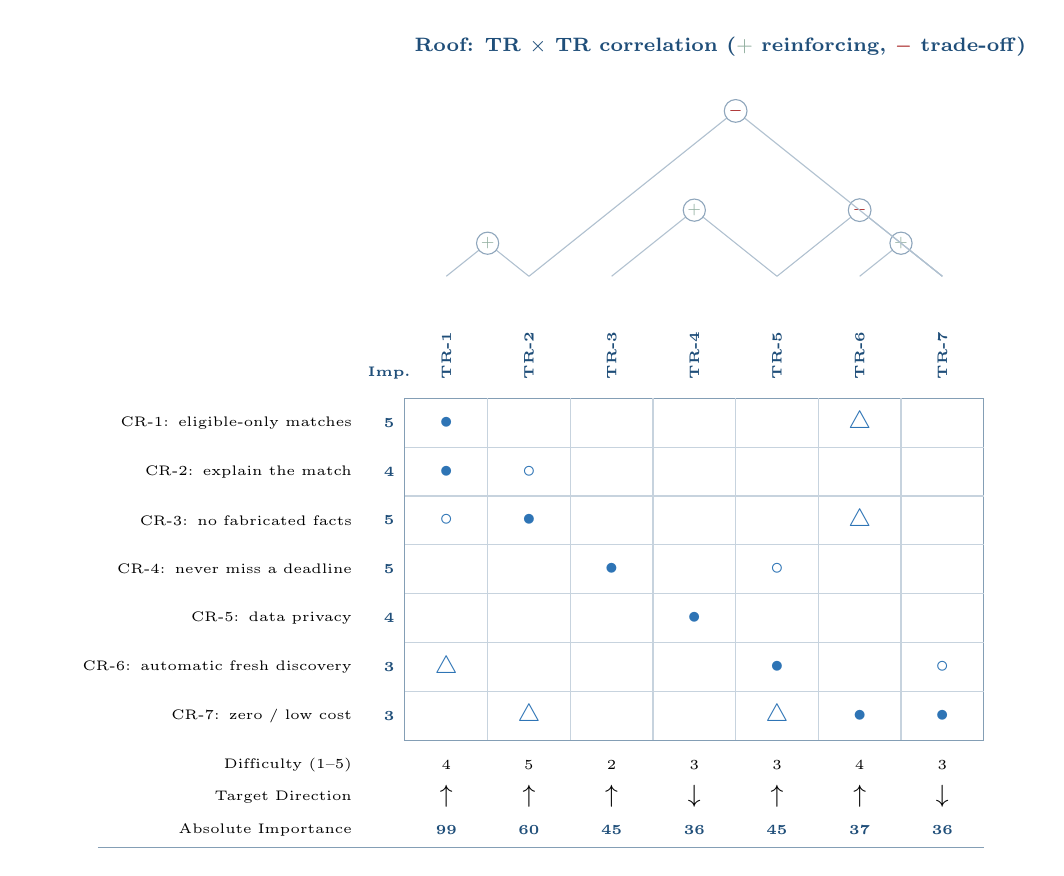
\begin{tikzpicture}[x=1cm,y=1cm,font=\tiny]
  % ---- geometry ----
  % 7 columns (TR1..TR7), width 1.05cm each; 7 rows (CR1..CR7), height 0.62cm each
  \def\cw{1.05}
  \def\rh{0.62}
  % column centers
  \foreach \i in {1,...,7}{\pgfmathsetmacro{\cx}{(\i-0.5)*\cw}\expandafter\xdef\csname cx\i\endcsname{\cx}}

  % ---- roof (correlation triangle) ----
  \def\roofbase{1.55}
  \foreach \i/\j/\lvl/\sym/\col in {1/2/1/{\qpos}/{nodegreen!70!black},
                                     6/7/1/{\qpos}/{nodegreen!70!black},
                                     3/5/2/{\qpos}/{nodegreen!70!black},
                                     5/7/2/{\qneg}/{red!60!black},
                                     2/7/5/{\qneg}/{red!60!black}}{
    \pgfmathsetmacro{\xi}{(\i-0.5)*\cw}
    \pgfmathsetmacro{\xj}{(\j-0.5)*\cw}
    \pgfmathsetmacro{\xm}{(\xi+\xj)/2}
    \pgfmathsetmacro{\ym}{\roofbase+\lvl*0.42}
    \draw[darkblue!35,thin] (\xi,\roofbase) -- (\xm,\ym) -- (\xj,\roofbase);
    \node[circle,draw=darkblue!50,fill=white,inner sep=0.5pt,font=\tiny] at (\xm,\ym) {\sym};
  }
  \node[font=\scriptsize\bfseries,darkblue,anchor=south west] at (0,\roofbase+6*0.42+0.15)
    {Roof: TR $\times$ TR correlation (\qpos\ reinforcing, \qneg\ trade-off)};

  % ---- column headers (rotated) ----
  \foreach \i/\lbl in {1/TR-1,2/TR-2,3/TR-3,4/TR-4,5/TR-5,6/TR-6,7/TR-7}{
    \pgfmathsetmacro{\cx}{(\i-0.5)*\cw}
    \node[font=\tiny\bfseries,darkblue,anchor=west,rotate=90] at (\cx,0.12) {\lbl};
  }

  % ---- grid ----
  \draw[darkblue!55] (0,0) rectangle (7*\cw,-7*\rh);
  \foreach \i in {1,...,6}{\draw[darkblue!25] (\i*\cw,0) -- (\i*\cw,-7*\rh);}
  \foreach \j in {1,...,6}{\draw[darkblue!25] (0,-\j*\rh) -- (7*\cw,-\j*\rh);}

  % ---- row labels + importance weights ----
  \foreach \j/\lbl/\imp in {1/{CR-1: eligible-only matches}/5,
                             2/{CR-2: explain the match}/4,
                             3/{CR-3: no fabricated facts}/5,
                             4/{CR-4: never miss a deadline}/5,
                             5/{CR-5: data privacy}/4,
                             6/{CR-6: automatic fresh discovery}/3,
                             7/{CR-7: zero / low cost}/3}{
    \pgfmathsetmacro{\cy}{-(\j-0.5)*\rh}
    \node[font=\tiny,anchor=east,text width=4.0cm,align=right] at (-0.55,\cy) {\lbl};
    \node[font=\tiny\bfseries,darkblue,anchor=center] at (-0.2,\cy) {\imp};
  }
  \node[font=\tiny\bfseries,darkblue,anchor=south] at (-0.2,0.12) {Imp.};

  % ---- relationship symbols ----
  \foreach \j/\i/\sym in {1/1/{\qstrong},1/6/{\qweak},
                           2/1/{\qstrong},2/2/{\qmed},
                           3/2/{\qstrong},3/1/{\qmed},3/6/{\qweak},
                           4/3/{\qstrong},4/5/{\qmed},
                           5/4/{\qstrong},
                           6/5/{\qstrong},6/7/{\qmed},6/1/{\qweak},
                           7/7/{\qstrong},7/6/{\qstrong},7/2/{\qweak},7/5/{\qweak}}{
    \pgfmathsetmacro{\cx}{(\i-0.5)*\cw}
    \pgfmathsetmacro{\cy}{-(\j-0.5)*\rh}
    \node[font=\small] at (\cx,\cy) {\sym};
  }

  % ---- bottom summary rows ----
  \draw[darkblue!55] (0,-7*\rh) -- (7*\cw,-7*\rh);
  \foreach \i/\diff in {1/4,2/5,3/2,4/3,5/3,6/4,7/3}{
    \pgfmathsetmacro{\cx}{(\i-0.5)*\cw}
    \node[font=\tiny] at (\cx,-7*\rh-0.32) {\diff};
  }
  \node[font=\tiny,anchor=east,text width=4.0cm,align=right] at (-0.55,-7*\rh-0.32) {Difficulty (1--5)};

  \foreach \i/\dir in {1/{$\uparrow$},2/{$\uparrow$},3/{$\uparrow$},4/{$\downarrow$},5/{$\uparrow$},6/{$\uparrow$},7/{$\downarrow$}}{
    \pgfmathsetmacro{\cx}{(\i-0.5)*\cw}
    \node[font=\small] at (\cx,-7*\rh-0.72) {\dir};
  }
  \node[font=\tiny,anchor=east,text width=4.0cm,align=right] at (-0.55,-7*\rh-0.72) {Target Direction};

  \foreach \i/\imp in {1/99,2/60,3/45,4/36,5/45,6/37,7/36}{
    \pgfmathsetmacro{\cx}{(\i-0.5)*\cw}
    \node[font=\tiny\bfseries,darkblue] at (\cx,-7*\rh-1.14) {\imp};
  }
  \node[font=\tiny,anchor=east,text width=4.0cm,align=right] at (-0.55,-7*\rh-1.14) {Absolute Importance};
  \draw[darkblue!55] (-3.9,-7*\rh-1.36) -- (7*\cw,-7*\rh-1.36);
\end{tikzpicture}
\end{center}
\captionof{figure}{House of Quality relating customer requirements (rows) to engineering
requirements (columns). Legend: \qstrong\ strong (9), \qmed\ moderate (3), \qweak\ weak (1);
roof symbols \qpos/\qneg\ mark reinforcing/conflicting technical trade-offs.}

\noindent\textbf{Reading the matrix.} TR-1 (hybrid semantic + GraphRAG eligibility scoring)
carries the highest absolute importance (99), which is why matching is built as a fused
score with a hard eligibility gate rather than similarity ranking alone (\S\ref{sec:reqlist},
FR-6). The roof also surfaces a genuine tension the design has to manage explicitly: the
Quality-Gate fact-check loop (TR-2) and the free-tier cost bound (TR-7) pull against each
other, because every retry the gate demands is an extra paid or rate-limited inference call
--- this is why NFR-4 caps page counts and paces requests rather than leaving the retry
budget unbounded.

% ══════════════════════════════════════════════════════════════════════════════
\section{Requirements Modeling}
This section models the functional requirements of \S\ref{sec:reqlist} as UML views: a use
case diagram for scope and actors, an activity diagram for the primary end-to-end workflow, a
sequence diagram for the highest-risk interaction (grounded drafting), and low-fidelity
wireframes as an early prototype of the resulting screens.

\subsection{Use Case Diagram}
The Applicant is the only human actor; a Scheduler (a cron-triggered system actor) is the
sole non-human actor, standing in for the daily automated re-search that FR-11 requires
without any user action.

% local styles for this diagram only
\tikzset{
  uc/.style={ellipse,draw=darkblue!60,fill=nodeblue,align=center,font=\tiny,
             inner sep=3pt,minimum width=2.7cm,minimum height=0.9cm},
  ucx/.style={uc,fill=nodegreen,minimum width=2.3cm,minimum height=0.75cm},
}
\newcommand{\stickfig}[2]{% (x,y) label
  \begin{scope}[shift={#1}]
    \draw[darkblue!75,line width=0.7pt] (0,1.05) circle (0.17);
    \draw[darkblue!75,line width=0.7pt] (0,0.88) -- (0,0.25);
    \draw[darkblue!75,line width=0.7pt] (-0.32,0.72) -- (0,0.88) -- (0.32,0.72);
    \draw[darkblue!75,line width=0.7pt] (-0.28,-0.15) -- (0,0.25) -- (0.28,-0.15);
    \node[font=\scriptsize\bfseries,darkblue,align=center] at (0,-0.45) {#2};
  \end{scope}
}

\begin{center}
\begin{tikzpicture}[x=1cm,y=1cm]
  % system boundary
  \draw[darkblue!55,rounded corners=4pt] (1.7,0.3) rectangle (11.1,9.1);
  \node[font=\scriptsize\bfseries,darkblue] at (6.4,8.75) {scholar-agent Platform};

  % use cases -- column A (x=4.2) and column B (x=8.6)
  \node[uc] (uc1) at (4.2,7.9) {Register \&\\Authenticate};
  \node[uc] (uc2) at (8.6,7.9) {Manage CV\\Profile};
  \node[uc] (uc3) at (4.2,6.5) {Discover\\Opportunities};
  \node[uc] (uc4) at (8.6,6.5) {Browse \& Filter\\Catalog};
  \node[uc] (uc5) at (4.2,5.1) {Track\\Application};
  \node[uc] (uc6) at (8.6,5.1) {Draft Application\\Materials};
  \node[uc] (uc7) at (4.2,3.7) {Manage Professor\\Outreach};
  \node[uc] (uc8) at (8.6,3.7) {Export\\Calendar};
  \node[uc] (uc9) at (4.2,2.3) {Manage\\Watchlist};
  \node[uc] (uc10) at (8.6,2.3) {Practice Writing\\(Studio)};
  \node[ucx] (uc11) at (4.2,1.0) {Auto-Surf\\Watchlist};

  % actors
  \stickfig{(-0.9,3.6)}{Applicant}
  \stickfig{(12.0,0.5)}{Scheduler\\{\scriptsize\itshape (cron)}}

  % actor associations
  \foreach \t in {uc1,uc2,uc3,uc4,uc5,uc6,uc7,uc8,uc9,uc10}{
    \draw[darkblue!55,thin] (-0.35,4.05) -- (\t.west);
  }
  \draw[darkblue!55,thin] (12.0,1.0) -- (uc11.east);

  % include / extend
  \draw[dashed,-{Stealth[length=1.8mm]},darkblue!70] (uc11) to node[font=\tiny,fill=white,inner sep=1pt]{$\ll$extend$\gg$} (uc9);
  \draw[dashed,-{Stealth[length=1.8mm]},darkblue!70] (uc3) to[bend right=12] node[font=\tiny,fill=white,inner sep=1pt,pos=0.5]{$\ll$include$\gg$} (uc4.north west |- uc3);
\end{tikzpicture}
\end{center}
\captionof{figure}{Use case diagram. The Applicant drives every top-level function; the
Scheduler actor triggers \emph{Auto-Surf Watchlist}, which \emph{extends} \emph{Manage
Watchlist} (FR-11) instead of requiring a manual search each day.}

\noindent Note on \emph{Discover Opportunities}: a manual, free-text search
(\emph{include}s the same extraction pipeline the Scheduler triggers automatically) and the
scheduled surf are two entry points into one underlying use case, which is why they share the
extraction and de-duplication logic behind FR-3/FR-4 rather than each implementing it
separately.

\subsection{Activity Diagram}
The activity diagram below traces the primary end-to-end workflow --- from CV upload to a
tracked, drafted application --- across the two swimlanes that matter to the requirements:
what the Applicant does, and what the System does on their behalf. The two decision points
correspond directly to FR-6 (the match threshold) and FR-8 (the groundedness check that
EX-1 requires before a draft is ever shown).

\tikzset{
  aact/.style={rectangle,rounded corners=3pt,draw=darkblue!55,fill=nodeindigo,
               align=center,font=\tiny,inner sep=3pt,minimum width=3.0cm,minimum height=0.75cm},
  sact/.style={rectangle,rounded corners=3pt,draw=darkblue!55,fill=nodegreen,
               align=center,font=\tiny,inner sep=3pt,minimum width=3.1cm,minimum height=0.75cm},
  dec/.style={diamond,draw=darkblue!55,fill=nodegray,align=center,font=\tiny,
              inner sep=1pt,aspect=2.2,minimum width=3.0cm},
}

\begin{center}
\begin{tikzpicture}[x=1cm,y=1cm,>=Stealth]
  % swimlane bands
  \begin{scope}[on background layer]
    \fill[titleblue!5] (0.1,-0.3) rectangle (4.1,12.1);
    \fill[nodegreen!25] (4.1,-0.3) rectangle (10.6,12.1);
  \end{scope}
  \draw[darkblue!40] (4.1,-0.3) -- (4.1,12.1);
  \node[font=\scriptsize\bfseries,darkblue] at (2.1,11.85) {Applicant};
  \node[font=\scriptsize\bfseries,darkblue] at (7.3,11.85) {System (Discovery Engine / API)};

  % nodes
  \node[circle,fill=darkblue,minimum size=0.28cm] (start) at (2.1,11.2) {};
  \node[aact] (a1) at (2.1,10.3) {Upload / paste CV};
  \node[sact] (s1) at (7.3,10.3) {Extract structured profile};
  \node[sact] (s2) at (7.3,9.1)  {Search web \& extract opportunities};
  \node[sact] (s3) at (7.3,7.9)  {Score \& rank vs.\ profile};
  \node[dec]  (d1) at (7.3,6.5)  {Eligible \&\\score $\geq$ threshold?};
  \node[sact] (s4) at (7.3,5.2)  {Present match + rationale};
  \node[aact] (a2) at (2.1,5.2)  {Review \& save to pipeline};
  \node[aact] (a3) at (2.1,4.0)  {Request draft\\(email + SOP)};
  \node[sact] (s5) at (7.3,4.0)  {Generate grounded draft};
  \node[dec]  (d2) at (7.3,2.6)  {Groundedness\\check passes?};
  \node[sact] (s6) at (10.0,2.6) {Rewrite with\\Quality-Gate feedback};
  \node[sact] (s7) at (7.3,1.3)  {Persist documents; update status \& deadlines};
  \node[aact] (a4) at (2.1,1.3)  {Export calendar / follow up};
  \node[circle,fill=darkblue,minimum size=0.28cm] (endn) at (2.1,0.2) {};
  \draw[darkblue,line width=0.6pt] (2.1,0.2) circle (0.19cm);

  % flow
  \draw[fl] (start) -- (a1);
  \draw[fl] (a1) -- (s1);
  \draw[fl] (s1) -- (s2);
  \draw[fl] (s2) -- (s3);
  \draw[fl] (s3) -- (d1);
  \draw[fl] (d1) -- node[right,font=\tiny]{yes} (s4);
  \draw[fl] (d1.west) to[bend left=45] node[left,font=\tiny,align=center]{no (next\\opportunity)} (s3.west);
  \draw[fl] (s4) -- (a2);
  \draw[fl] (a2) -- (a3);
  \draw[fl] (a3) -- (s5);
  \draw[fl] (s5) -- (d2);
  \draw[fl] (d2) -- node[above,font=\tiny]{no} (s6);
  \draw[fl] (s6.north) to[bend left=35] node[right,font=\tiny]{retry $\leq N$} (d2.east);
  \draw[fl] (d2) -- node[left,font=\tiny]{yes} (s7);
  \draw[fl] (s7) -- (a4);
  \draw[fl] (a4) -- (endn);
\end{tikzpicture}
\end{center}
\captionof{figure}{Activity diagram for the end-to-end discovery-to-drafting workflow, with
swimlanes separating Applicant actions from System actions.}

\subsection{Sequence Diagram}
The sequence below models FR-8, the highest-risk interaction in the system: it is the one
place a fabricated fact could reach the professor, which is exactly why EX-1's Quality-Gate
loop sits directly in this call path rather than being an optional post-check.

\tikzset{
  life/.style={draw=darkblue!55,dashed},
  actb/.style={rectangle,draw=darkblue!55,fill=nodeblue,inner sep=0pt,minimum width=0.14cm},
  lhead/.style={rectangle,rounded corners=2pt,draw=darkblue!55,fill=nodeindigo,
                font=\tiny\bfseries,align=center,inner sep=3pt,minimum width=1.9cm},
}

\begin{center}
\begin{tikzpicture}[x=1cm,y=1cm,font=\tiny,>=Stealth]
  % lifeline x-positions
  \def\xA{0.4}   % Applicant
  \def\xU{2.7}   % Web UI
  \def\xP{5.2}   % API controller
  \def\xS{7.9}   % Assistant Service
  \def\xL{10.6}  % LLM Gateway
  \def\xR{13.1}  % Repository

  % headers
  \node[lhead] (hA) at (\xA,11.6) {Applicant};
  \node[lhead] (hU) at (\xU,11.6) {Web UI};
  \node[lhead] (hP) at (\xP,11.6) {API\\(\code{me} controller)};
  \node[lhead] (hS) at (\xS,11.6) {Assistant\\Service};
  \node[lhead] (hL) at (\xL,11.6) {LLM\\Gateway};
  \node[lhead] (hR) at (\xR,11.6) {Repository};

  % lifelines
  \foreach \x in {\xA,\xU,\xP,\xS,\xL,\xR}{\draw[life] (\x,11.1) -- (\x,0.6);}

  % activation bars
  \draw[actb] (\xP-0.07,9.9) rectangle (\xP+0.07,2.05);
  \draw[actb] (\xS-0.07,9.3) rectangle (\xS+0.07,2.75);

  % messages
  \draw[fl] (\xA,10.6) -- node[above,font=\tiny]{click ``Draft email + SOP''} (\xU,10.6);
  \draw[fl] (\xU,9.9) -- node[above,font=\tiny]{POST /me/applications/\{id\}/draft} (\xP,9.9);
  \draw[fl] (\xP,9.3) -- node[above,font=\tiny]{draft\_application(app, profile)} (\xS,9.3);
  \draw[fl] (\xS,8.6) -- node[above,font=\tiny]{fetch profile, opportunity, professor record} (\xR,8.6);
  \draw[fl,dashed] (\xR,8.0) -- node[above,font=\tiny]{records} (\xS,8.0);

  % loop frame
  \draw[darkblue!50] (\xS-1.55,7.6) rectangle (\xL+1.15,4.55);
  \node[font=\tiny,darkblue,anchor=north west] at (\xS-1.55,7.6)
    {\textbf{loop} \,[until approved or retries $\leq$ N]};

  \draw[fl] (\xS,7.0) -- node[above,font=\tiny]{structured(complete): draft prompt} (\xL,7.0);
  \draw[fl,dashed] (\xL,6.4) -- node[above,font=\tiny]{ColdEmail + SOPDraft} (\xS,6.4);
  \draw[fl] (\xS,5.75) to[out=20,in=-20,looseness=6] node[right,font=\tiny,align=left]{Quality Gate:\\check groundedness} (\xS,5.2);
  \draw[fl,dashed] (\xS-1.35,4.85) -- node[below,font=\tiny,align=center,pos=0.5]{if not approved: feedback\\attached, loop repeats} (\xS-0.15,4.85);

  \draw[fl] (\xS,3.9) -- node[above,font=\tiny]{persist drafted documents on application} (\xR,3.9);
  \draw[fl,dashed] (\xR,3.35) -- node[above,font=\tiny]{ack} (\xS,3.35);
  \draw[fl,dashed] (\xS,2.75) -- node[above,font=\tiny]{SynthesisBundle} (\xP,2.75);
  \draw[fl,dashed] (\xP,2.05) -- node[above,font=\tiny]{200 OK + bundle} (\xU,2.05);
  \draw[fl,dashed] (\xU,1.3) -- node[above,font=\tiny]{render drafts (copy / download)} (\xA,1.3);
\end{tikzpicture}
\end{center}
\captionof{figure}{Sequence diagram for \emph{Draft Application Materials} (FR-8). The loop
fragment is where EX-1's anti-hallucination guarantee is actually enforced: no draft leaves
the Assistant Service until the Quality Gate approves it or the retry budget is exhausted.}

\subsection{Prototyping Using Wireframes / UI Sketches}
The wireframes below are the earliest concrete prototype of the requirements above: every
control on them exists because a specific FR calls for it, and nothing on them exists that
isn't traceable to one. They are intentionally low-fidelity (boxes and labels only) so that
review focuses on layout and interaction, not on final visual styling.

% wireframe primitives
\tikzset{
  wframe/.style={rectangle,draw=darkblue!45,fill=white,line width=0.4pt},
  wbar/.style={rectangle,draw=darkblue!35,fill=nodeindigo!70,font=\tiny,inner sep=2pt,align=center},
  wfield/.style={rectangle,draw=darkblue!35,fill=gray!8,font=\tiny,inner sep=2pt,align=left},
  wbtn/.style={rectangle,rounded corners=2pt,draw=darkblue!50,fill=titleblue!25,font=\tiny,inner sep=2pt,align=center},
  wchip/.style={rectangle,rounded corners=3pt,draw=darkblue!30,fill=nodeblue,font=\tiny,inner sep=1.6pt},
  wcard/.style={rectangle,rounded corners=2pt,draw=darkblue!30,fill=gray!5,font=\tiny,align=left,inner sep=2.5pt},
  wlab/.style={font=\tiny,gray},
}

\subsubsection{Wireframe 1: Application Tracker (home) --- realises FR-7}
The home screen is a Kanban board with one column per pipeline stage. A fixed top bar carries
the brand, page navigation, a calendar-export action, and the account menu. Cards are dragged
between columns to change status.

\begin{center}
\begin{tikzpicture}[x=1cm,y=1cm]
  \draw[wframe] (0,0) rectangle (12,6.4);
  % top bar
  \node[wbar,minimum width=11.6cm,minimum height=0.5cm,anchor=north west] at (0.2,6.2)
    {};
  \node[font=\tiny\bfseries,anchor=west] at (0.35,5.95) {scholar$\cdot$agent};
  \foreach \i/\t in {0/Tracker,1/Browse,2/Discover,3/Build KB,4/Studio}{
    \node[font=\tiny,anchor=west] at (2.5+\i*1.35,5.95) {\t};}
  \node[wbtn,anchor=east] at (10.8,5.95) {Calendar};
  \node[font=\tiny,anchor=east] at (11.8,5.95) {user\,$\vee$};
  % column headers + cards
  \foreach \i/\h in {0/Interested,1/Preparing,2/Applied,3/Interview}{
    \node[wbar,minimum width=2.6cm,minimum height=0.4cm,anchor=north west] at (0.25+\i*2.9,5.4) {\h};}
  % a few cards
  \node[wcard,minimum width=2.5cm,minimum height=0.85cm,anchor=north west] at (0.3,4.85)
    {\textbf{DAAD PhD}\\TU Munich\\{\color{red!70}$\odot$ soon}};
  \node[wcard,minimum width=2.5cm,minimum height=0.85cm,anchor=north west] at (0.3,3.85)
    {\textbf{Chevening}\\UK};
  \node[wcard,minimum width=2.5cm,minimum height=0.85cm,anchor=north west] at (3.2,4.85)
    {\textbf{Erasmus MSc}\\$\odot$ Nov 1};
  \node[wcard,minimum width=2.5cm,minimum height=0.85cm,anchor=north west] at (6.1,4.85)
    {\textbf{Fulbright}\\applied};
  \node[wbtn,anchor=north east] at (11.75,5.4) {+ Add manually};
  \node[wlab,anchor=south west] at (0.25,0.1) {Drag a card between columns to change its status.};
\end{tikzpicture}
\end{center}

\subsubsection{Wireframe 2: Application Detail Drawer --- realises FR-7, FR-8}
Clicking a card slides in a right-hand drawer (an in-place sub-state, not a new page). It
holds the status and deadline controls, a requirement checklist, a \emph{Materials} section
whose ``Draft email + SOP'' button generates and persists documents (FR-8), and a notes field.

\begin{center}
\begin{tikzpicture}[x=1cm,y=1cm]
  \draw[wframe] (0,0) rectangle (12,5.6);
  \fill[gray!4] (0,0) rectangle (7.4,5.6);
  \node[wlab] at (3.7,2.8) {(tracker board behind, dimmed)};
  % drawer
  \draw[wframe,fill=gray!2] (7.4,0) rectangle (12,5.6);
  \node[font=\tiny\bfseries,anchor=north west] at (7.55,5.45) {DAAD PhD, TU Munich};
  \node[font=\tiny,anchor=north east] at (11.85,5.45) {$\times$};
  \node[wfield,minimum width=2.1cm,anchor=north west] at (7.55,4.85) {Status: Preparing $\vee$};
  \node[wfield,minimum width=2.0cm,anchor=north west] at (9.75,4.85) {Deadline: 2026-11-01};
  \node[font=\tiny\bfseries,anchor=north west] at (7.55,4.35) {Checklist};
  \foreach \i/\c/\t in {0/$\boxtimes$/CV,1/$\square$/SOP,2/$\square$/IELTS}{
    \node[font=\tiny,anchor=north west] at (7.55+\i*1.3,4.05) {\c\ \t};}
  \node[font=\tiny\bfseries,anchor=north west] at (7.55,3.5) {Materials};
  \node[wbtn,anchor=north east] at (11.85,3.55) {Draft email + SOP};
  \node[wcard,minimum width=4.2cm,anchor=north west] at (7.55,3.1) {$\triangleright$ PhD inquiry (Email)\quad copy $\cdot$ download};
  \node[wcard,minimum width=4.2cm,anchor=north west] at (7.55,2.55) {$\triangleright$ Statement of Purpose (SOP)};
  \node[wfield,minimum width=4.2cm,minimum height=0.8cm,anchor=north west] at (7.55,1.95) {Notes\ldots};
  \node[wbtn,anchor=south west] at (7.55,0.15) {Save changes};
  \node[font=\tiny,anchor=south east] at (11.85,0.15) {Cancel};
\end{tikzpicture}
\end{center}

\subsubsection{Wireframe 3: Browse Catalog and Writing Studio --- realises FR-5, FR-12}
Two further screens are shown together. Browse is a filtered card grid over the knowledge
base (FR-5); the Studio is a two-panel practice screen (input left, scored feedback right)
that realises the criterion-level scoring of FR-12.

\begin{center}
\begin{tikzpicture}[x=1cm,y=1cm]
  % --- Browse ---
  \draw[wframe] (0,0) rectangle (5.7,5.4);
  \node[font=\tiny\bfseries,anchor=north west] at (0.15,5.3) {Browse};
  \node[wfield,minimum width=5.3cm,anchor=north west] at (0.2,4.9) {search title / university\ldots};
  \foreach \i/\t in {0/Scholarships,1/PhD,2/Fellowship}{
    \node[wchip,anchor=north west] at (0.2+\i*1.55,4.35) {\t};}
  \node[wchip,anchor=north west,fill=nodegreen] at (4.15,4.35) {Funded};
  \foreach \r in {0,1}{\foreach \c in {0,1,2}{
    \node[wcard,minimum width=1.6cm,minimum height=1.1cm,anchor=north west]
      at (0.2+\c*1.78,3.85-\r*1.35) {\textbf{Title}\\Univ.\\$\odot$ date\\{\color{titleblue}Save}};}}
  \node[wlab,anchor=south west] at (0.2,0.1) {3-col grid (1-col on mobile)};
  % --- Studio ---
  \draw[wframe] (6.3,0) rectangle (12,5.4);
  \node[font=\tiny\bfseries,anchor=north west] at (6.45,5.3) {Writing Studio};
  % left input
  \foreach \i/\t in {0/{IELTS T2},1/{T1},2/SOP,3/Acad.}{
    \node[wchip,anchor=north west] at (6.45+\i*0.9,4.85) {\t};}
  \node[wfield,minimum width=2.5cm,minimum height=0.5cm,anchor=north west] at (6.45,4.3) {task prompt\ldots};
  \node[wfield,minimum width=2.5cm,minimum height=1.6cm,anchor=north west] at (6.45,3.7) {your essay\ldots\\\\{\color{gray}142 words}};
  \node[wbtn,anchor=north west] at (6.45,1.95) {Assess};
  % right feedback
  \node[circle,draw=titleblue,fill=nodegreen,minimum size=0.9cm,font=\tiny,anchor=north west] at (9.3,4.85) {6.5};
  \node[wlab,anchor=north west] at (10.35,4.75) {overall band};
  \foreach \i/\t/\sc in {0/Task/6.0, 1/Coherence/6.5, 2/Lexis/6.5, 3/Grammar/7.0}{
    \node[wcard,minimum width=2.3cm,anchor=north west] at (9.3,4.0-\i*0.42) {\t\hfill {\color{titleblue}\sc}};}
  \node[wcard,minimum width=2.5cm,anchor=north west] at (9.3,2.1) {$\checkmark$ strengths / $\blacktriangle$ fixes};
\end{tikzpicture}
\end{center}

\subsubsection{Screen Flow}
Authentication is the single entry gate: every other screen needs a valid session and
otherwise redirects to sign-in. The Tracker is the hub the other prototyped screens branch
off from, which is why it was sketched first and in the most detail.

\begin{center}
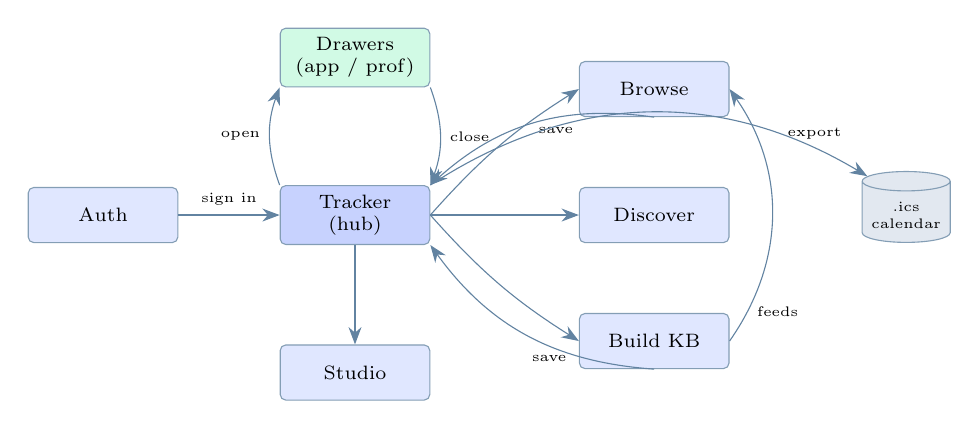
\begin{tikzpicture}[x=1cm,y=1cm,font=\scriptsize]
  \tikzset{nn/.style={rectangle,rounded corners=2pt,draw=darkblue!55,fill=nodeblue,
           minimum width=1.9cm,minimum height=0.7cm,align=center,font=\scriptsize},
           hub/.style={nn,fill=nodeindigo},
           sub/.style={nn,fill=nodegreen},
           st/.style={cylinder,shape border rotate=90,aspect=0.22,draw=darkblue!55,
                      fill=nodegray,font=\tiny,minimum height=0.9cm,align=center}}
  \node[nn] (auth) at (0,2) {Auth};
  \node[hub] (track) at (3.2,2) {Tracker\\(hub)};
  \node[sub] (draw) at (3.2,4) {Drawers\\(app / prof)};
  \node[nn] (browse) at (7,3.6) {Browse};
  \node[nn] (disc)   at (7,2)   {Discover};
  \node[nn] (build)  at (7,0.4) {Build KB};
  \node[nn] (studio) at (3.2,0) {Studio};
  \node[st] (cal)    at (10.2,2) {.ics\\calendar};
  \draw[fl] (auth) -- node[above,font=\tiny]{sign in} (track);
  \draw[fl] (track.north west) to[bend left=20] node[left,font=\tiny]{open} (draw.south west);
  \draw[fl] (draw.south east) to[bend left=20] node[right,font=\tiny]{close} (track.north east);
  \draw[fl] (track.east) to[bend left=8] (browse.west);
  \draw[fl] (track.east) -- (disc.west);
  \draw[fl] (track.east) to[bend right=8] (build.west);
  \draw[fl] (browse.south) to[bend right=25] node[below,font=\tiny,pos=.4]{save} (track.north east);
  \draw[fl] (build.south) to[bend left=25] node[below,font=\tiny,pos=.4]{save} (track.south east);
  \draw[fl] (build.east) to[bend right=35] node[right,font=\tiny,pos=.12]{feeds} (browse.east);
  \draw[fl] (track.south) -- (studio.north);
  \draw[fl] (track.north east) to[bend left=32] node[above,font=\tiny,pos=.88]{export} (cal.north west);
\end{tikzpicture}
\end{center}
\captionof{figure}{Screen flow across the prototyped wireframes. The Tracker is the hub;
authentication is the single gate; drawers are in-place sub-states rather than new pages.}

\vfill
\begin{center}\small\itshape End of Software Requirements Specification.\end{center}

\end{document}
